
\documentclass[10pt,journal,cspaper,compsoc]{IEEEtran}
\usepackage{amssymb}
\setcounter{tocdepth}{3}
\usepackage{graphicx}
\usepackage{subfig}
\usepackage{alltt}
\usepackage{amsmath}
\usepackage{url}
\usepackage{enumerate}
\usepackage{xspace}
\usepackage{tikz}

\usepackage{multirow}
\usepackage{times}
\usepackage{verbatim}

\usepackage{algorithm}
\usepackage[noend]{algorithmic}
\usepackage{caption}


\newtheorem{definition}{Definition}
\newtheorem{lemma}{Lemma}
\renewcommand{\labelitemii}{$\cdot$}
\newcommand{\gpu}{\textsc{GPU}\xspace}
\newcommand{\gpus}{\textsc{GPU}s}
\newcommand{\cpu}{\textsc{CPU}\xspace}
\newcommand{\cpus}{\textsc{CPU}s}
\newcommand{\cuda}{\textsc{Cuda}\xspace}
\newcommand{\oneexp}{1\textbf{EXP}\xspace}

\newcommand\bigo{\mathcal O}
\newtheorem{thm}{Theorem}
\newtheorem{corollary}[thm]{Corollary}

\DeclareMathOperator*{\argmin}{arg\,min}
\DeclareMathOperator*{\argmax}{arg\,max}


\hyphenation{op-tical net-works semi-conduc-tor}

\begin{document}
%
% paper title
% can use linebreaks \\ within to get better formatting as desired
\title{ Fast LRT Implementation \\on Parallel Computer Architectures}


% make the title area
\maketitle

\IEEEdisplaynotcompsoctitleabstractindextext

\IEEEpeerreviewmaketitle

\section{Motivations}
\label{sec:mov}

\subsection{Parallel Enumeration Schemes}
\label{sec:mov1}
In this section, we use a small example to demonstrate two different parallel strategies for performing LRT statistics in one-dimension data grid. The strategies are: (i) Overlapping Enumeration; (ii) Non-overlapping Enumeration. For simplicity, we will describe the strategies on GPGPU computing environment and they can be easily extended to multi-core and pc-clusters computing environments.

$\noindent \textit {Example:}$  A data set has five data points, denoted as $\{0,1,2,3,4\}$. Our task is how to enumerate all of the intervals among these five points in parallel. See Figure~\ref{example1}.

\begin{figure}[h]
\centering
\subfloat[Overlapping Enumeration]{
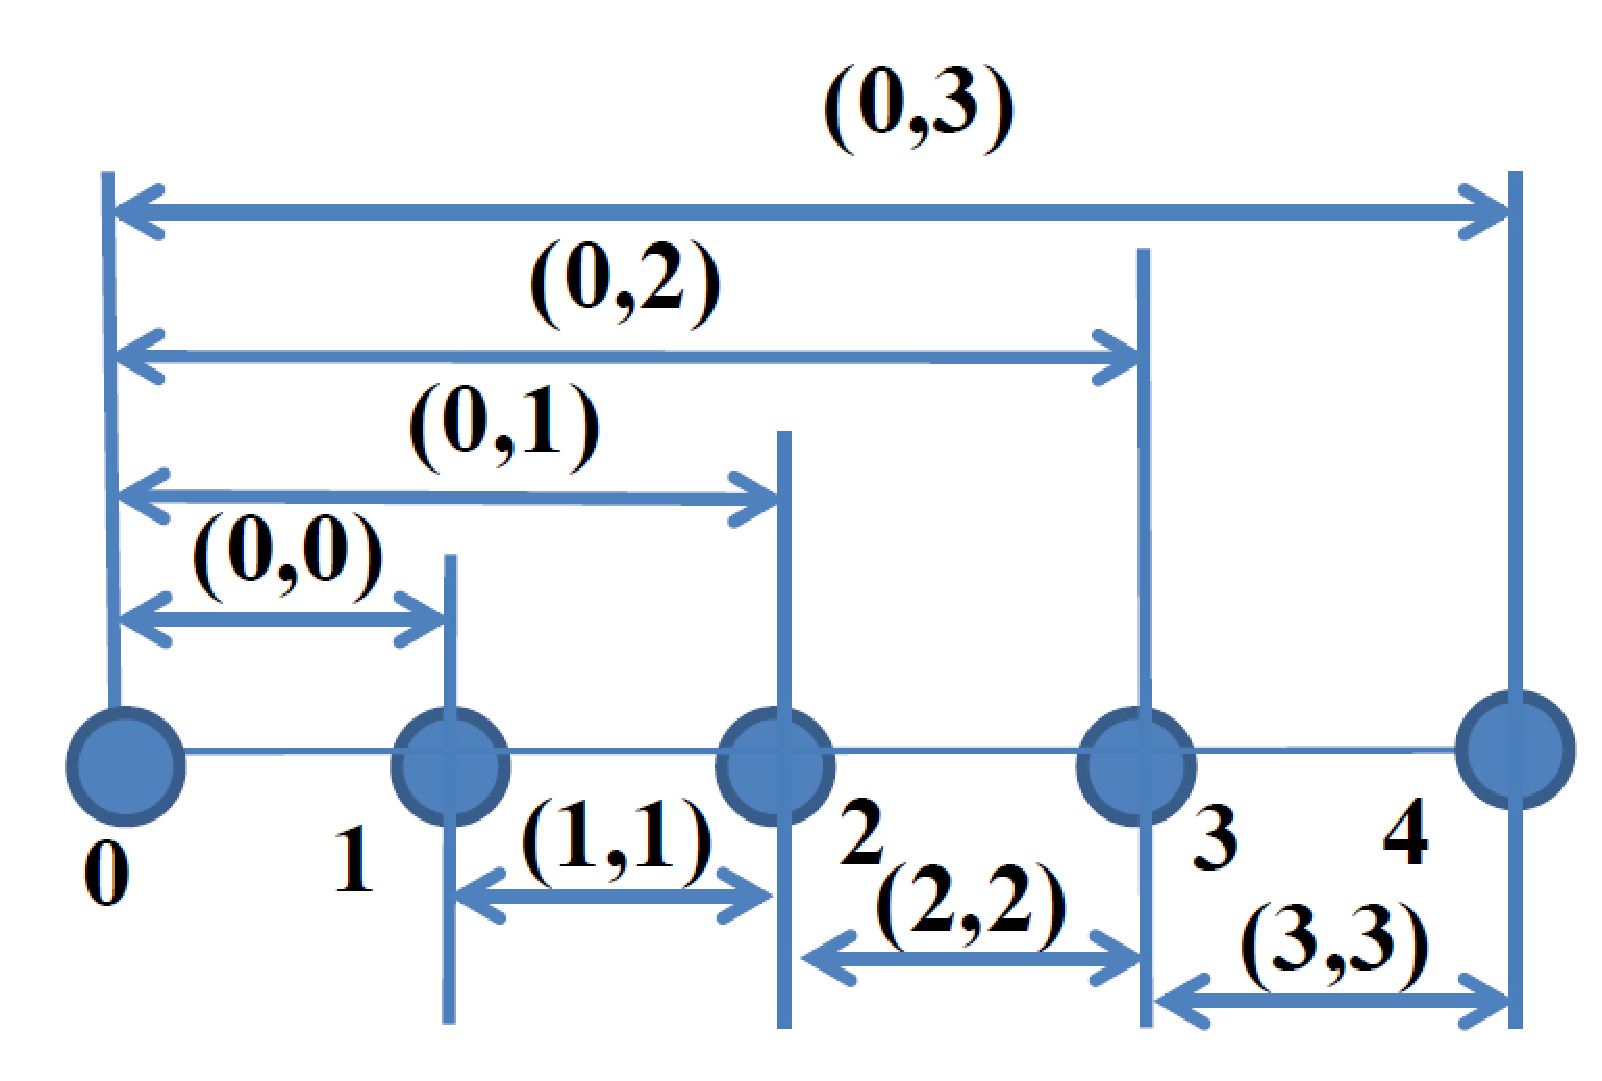
\includegraphics[width=0.5\linewidth]{figtkde/example11}
\label{example:subfig1}
}
~~\subfloat[Non-overlapping Enumeration]{
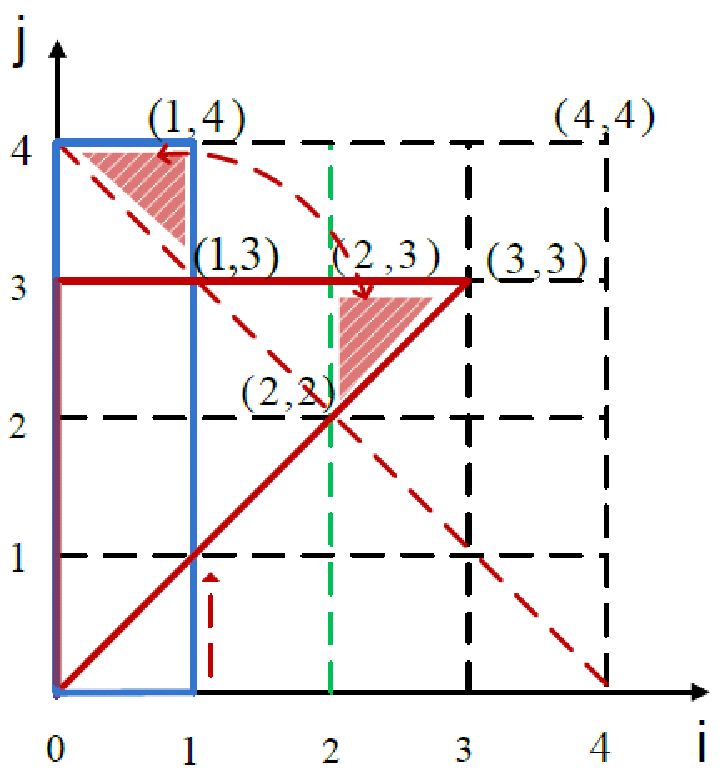
\includegraphics[width=0.4\linewidth]{figtkde/exampleven}
\label{example:subfig2}
}\\
\caption{Overlapping scheme and Non-overlapping scheme}\label{example1}
\end{figure}

 We express an interval between point $i_1$ and $i_2$ as $(i_1,i_2-1)$, where $i_2 > i_1$. We assume that each block can only maximally process $2$ intervals. The total number of intervals among five points is computed as: ${\frac{4 \cdot (4+1)}{2}}=2\times 5=10$.

  In the case of Overlapping Enumeration parallel strategy, every two overlapped intervals is assigned to a block. The next/previous interval always overlaps by one interval and the length of next interval is larger than previous interval.  From Figure~\ref{example1}(a), $\{(0,0),(0,1)\} \rightarrow$ block 0; $\{(1,1),(1,2)\} \rightarrow$block 1, we can see that the overlapping scheme enumerates all of the intervals up to size of two. However, some blocks may have fewer number of intervals when the last interval has been enumerated. For block 4, it has only one interval(i.e. $\{(3,3)\}$). This leads to an observation of workload unbalancing among blocks. Furthermore, in each block, different interval is assigned to different thread. The lengths of intervals are different and this can further creates different workload among different threads during brute-force calculation.

Interestingly, if we plot each interval between point $i_1$ and $i_2$ onto two-dimensional space, a triangular shape is formed. In Figure~\ref{example:subfig2}, all of the ten intervals forms a triangle shape enclosed by $\{(0,0)\rightarrow(3,3)\rightarrow(0,3)\}$. Furthermore, we notice that the total number of intervals can be treated as the product of $(n+1)$ and ${\frac{(n)}{2}}$. A rectangular shape can be formed by $(width,height)=(n+1,{\frac{n}{2}})$. In our example, $\{(0,0)\rightarrow(0,1)\rightarrow(1,4)\rightarrow(0,4)\}$ forms a rectangle and it has the exact same number of points as the formed triangular shape. Therefore, each point in this rectangle can be mapped to an interval. In a rectangular shape, we can divide the entire workload equally and assign each to each block. This solves the workload imbalance among blocks. In each block, each thread process the same number of intervals. However, this still does not solve the workload imbalance among each thread. In next section, we presents a dynamic programming scheme to pre-compute subsets of LRT statistic value and the computation of each thread becomes $O(1)$, which will solve the workload imbalance issue among threads.


The Overlapping Enumeration strategy has been implemented in [apweb]. In this paper, the Non-overlapping Enumeration strategy, called Range Mapping scheme, is presented to overcome the limitations of the Overlapping Enumeration strategy.

\subsection{Dynamic Pre-computation}
\label{sec:mov2}
The log-likelihood statistic (LRT) computation on 1EXP family is simplified to aggregate the statistic values from a given region $R$ (denoted as $\sum $), which is composed one or multiple cells. This makes

Consider Figure~\ref{fig:example}(a) showing a rectangular area $R$ embedded in a grid $G$. Instead of counting the number of elements in $R$ directly, we express set $R$ as set intersections of two sets $A$ and $B$ as shown in Figure~\ref{fig:example}(b). Set $A$ is a rectangular region that starts in the upper left corner of the grid and ends at the lower right corner of $R$. Set $B$ is a rectangular region that starts at the upper left corner of $R$ and ends at the lower right corner of the grid. Hence, $R=A \cap B$. We denote the region from the lower left corner of $G$ to the lower left corner of $R$ by $X$ and the region from the upper right corner of $R$ to the upper right corner of $G$ by $Y$.

\begin{figure}[h]
   \tikzset{oo grid/.style={help lines,color=blue!50!black!50,top color=white, opacity=0.5,bottom color=blue!50!black!20, very thick}}
     \begin{center}
     \begin{tikzpicture}

\draw [step=2pt][oo grid](0pt,0pt) rectangle (90pt,90pt);
\draw (10pt,80pt) node {G};
\draw [oo grid](20pt,30pt) rectangle (70pt,60pt);
\draw (45pt,45pt) node {R};

\draw [step=2pt] [oo grid](120pt,0pt) rectangle (210pt,90pt) ;

\draw [step=2pt][oo grid](140pt,30pt) rectangle (190pt,60pt);
\draw [step=2pt][oo grid](120pt,30pt) rectangle (190pt,90pt);
\draw [step=2pt][oo grid](140pt,0pt) rectangle (210pt,60pt);
\draw (130pt,80pt) node {G};
\draw (145pt,70pt) node {A};
\draw (165pt,45pt) node {R};
\draw (130pt,15pt) node {X};
\draw (200pt,75pt) node {Y};
\draw (185pt,15pt) node {B};

\draw (40pt,-15pt) node { (a) Region R in Grid G };
\draw (180pt,-15pt) node { (b) R= $A\cap B$ , $\overline{A}\cap\overline{B} = X \cup Y$};
\end{tikzpicture}
\end{center}
\vspace{-10pt}
\caption{Inclusive/Excusive Scheme}\label{fig:example}
\end{figure}



 By applying De Morgan's law and inclusion/exclusion principle, the query of counting the number of elements of region $R(x_1,y_1,x_2,y_2)$, where $(x_1,y_1)$ is the upper left corner and $(x_2,y_2)$ is the lower right corner is expressed by (see proof in appendix):

\small
\begin{equation}
\begin{split}
|R(x_1,y_1,x_2,y_2)|& = |A(x_2,y_2)| + |B(x_1,y_1)| + |X(x_1,y_2)| \\& \quad + |Y(x_2,y_1)| - |G|
\end{split}
\end{equation}
\normalsize
% that's all folks

\section{Range Mapping Scheme}
In this section, we study how parallelism helps to enumerate all of the rectangular regions (R) in a spatial grid (G).

From section~\ref{sec:mov1}, we know that if all of the pairwise intervals between $n$ data points, denoted as $(i,j)$, are plotted onto two-dimensional coordinate system, they form triangular shape. Each pair of $(i,j)$ in triangular-shaped space can be transformed to pair $(i',j')$ in rectangular-shaped space. After transformation, it enables the whole rectangular space to be partitioned into equal portions. Each portion consists of same amount of pairs and is distributed onto different ``parallel computing component'' (PCC) to balance workload and facilitate parallelization. We name this transforming scheme as range mapping scheme. This scheme can be directly extended to two dimensional spatial grid and multi-dimensional grid. We give details in the following:\\
Figure~\ref{trans:subfig1} plots out all of the intervals $(i,j)$ in two-dimensional space and we can see that these points $(i,j)$ forms a triangle. Figure~\ref{trans:subfig2} shows the rectangular-shaped space after transformation.
\begin{figure}[h]
\centering
\subfloat[]{
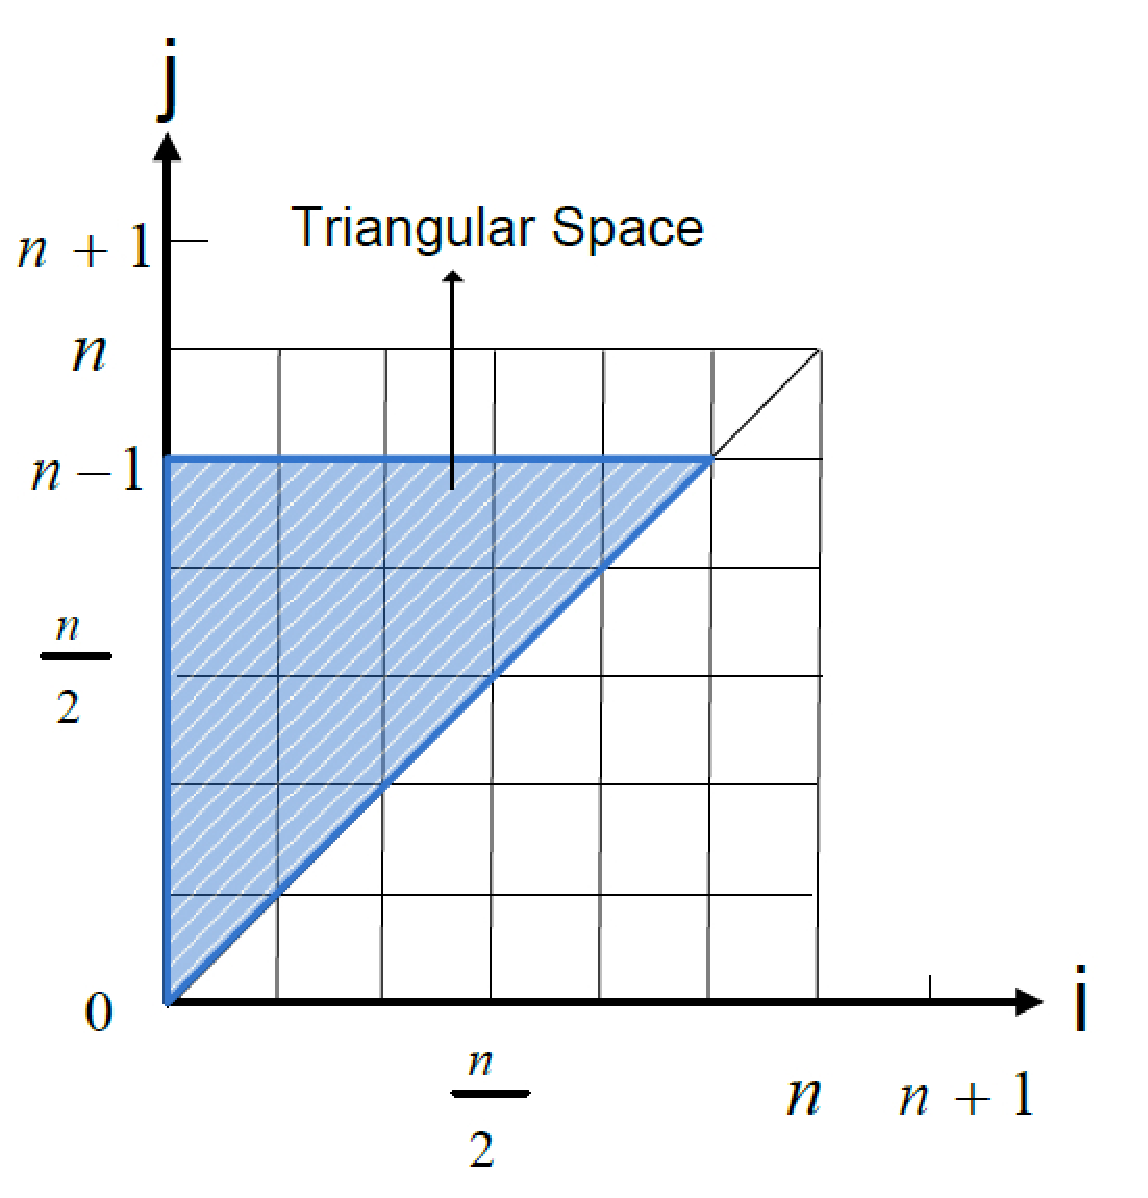
\includegraphics[width=0.45\linewidth]{figtkde/range1}
\label{trans:subfig1}
}
~~\subfloat[]{
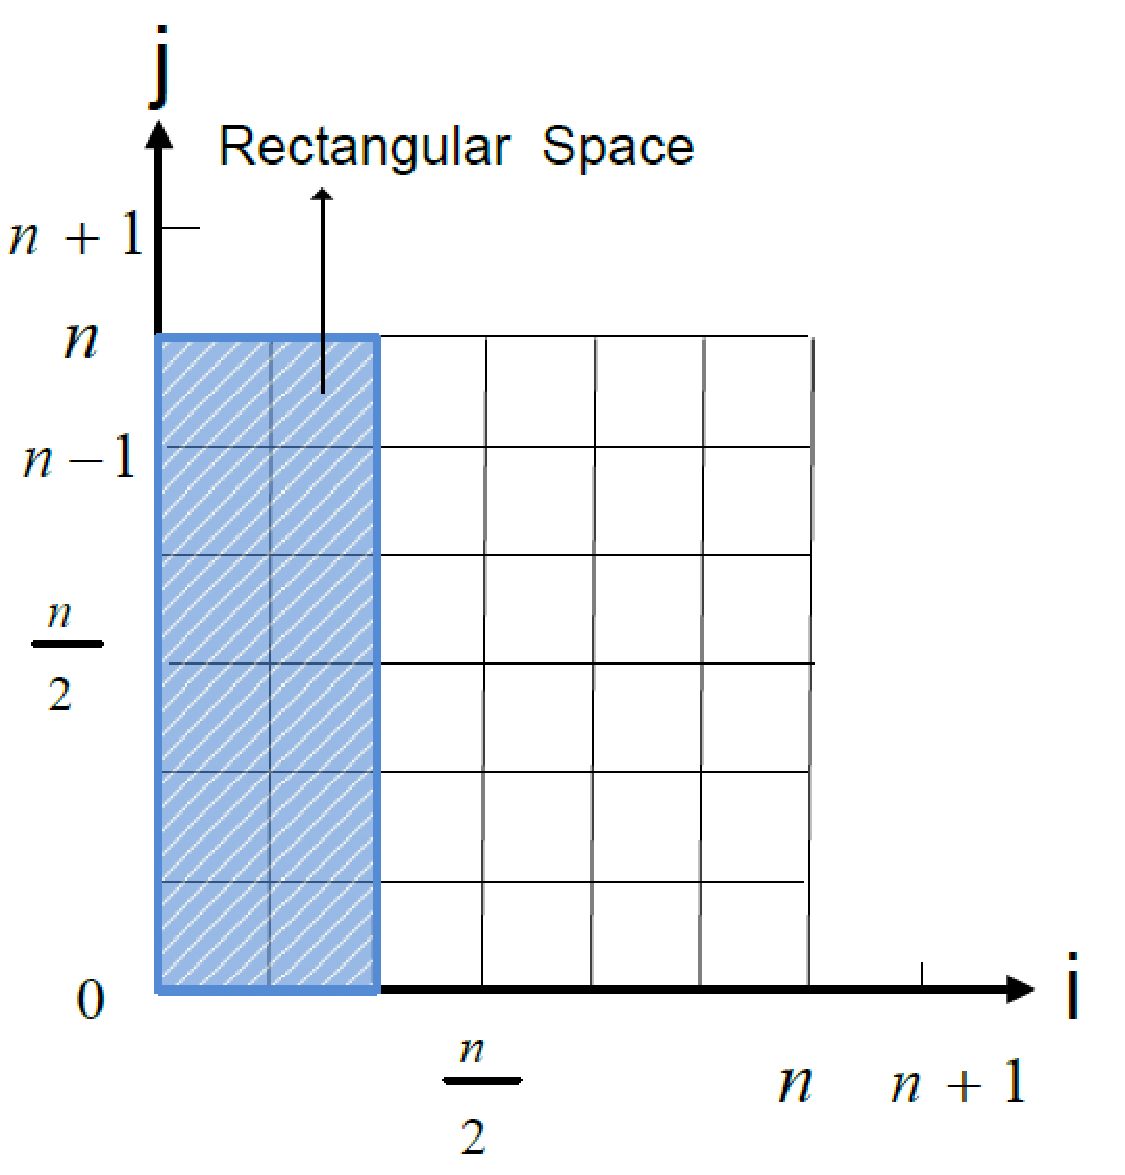
\includegraphics[width=0.45\linewidth]{figtkde/range2}
\label{trans:subfig2}
}
\caption{1-d Interval Transformation from $[n,n]$ to $[(n+1)/2,n]$}\label{modelBF}
\end{figure}

\subsection{One-Dimensional Mapping}
First, we consider the one-dimensional range mapping scheme. The axis oriented rectangles become intervals on one-dimensional space. We assume $n$ is the size of the data grid (i.e. array).\\

Given the following information:
\begin{flalign*}
&\mathbb N = \{0..n-1\}               & \\
&\mathbb R = \{0..\frac{n}{2}-1\} \times \{0..n\}     &\\
&\mathbb T = \{(i,j) \in \mathbb N^2 | i<=j\}   &\\
&\mathbb M = \{0.. \frac{n\times (n+1)}{2}-1\}  &\\
\end{flalign*}
where  $\mathbb N$ is coordinate range , $\mathbb R$ is rectangular space , $\mathbb T$ is triangular space  and $\mathbb M$ is number range of intervals.\\

\noindent There are two cases for the range mapping in one-dimensional grid: (1) The grid size $n$ is even (2) The grid size $n$ is odd. Please see the following:\\

\noindent \textbf{\textit{The grid size $n$ is even:}} Function $\phi: \mathbb M \rightarrow \mathbb R \rightarrow \mathbb T$ is composed of two mapping functions: $\phi_1: \mathbb M \rightarrow \mathbb R$ and $\phi_2: \mathbb R \rightarrow \mathbb T$. Firstly, $\phi_1$ transforms  $x\in \mathbb M$ to a pair in $(i,j)\in \mathbb R$ in rectangular space. Secondly, $\phi_2$ transforms the pair $(i,j)\in \mathbb R$ to a pair $(i',j')\in \mathbb T$ in triangular space.\\
\noindent\begin{definition}
Mapping Function
\begin{flalign*}
\phi_1:  \mathbb M \rightarrow \mathbb R & \\
x \mapsto (i,j)
\end{flalign*}
 where $i  = x / (n+1)$ and $j = x \mod (n+1)$.
\end{definition}
In this function, $x$ is an interval index and $(i,j)$ is mapped to $x$ by applying horner scheme.
 \vspace{5mm}
\begin{lemma}
The range of $\phi_1$ is $R$. That means: $i$ is in the range of  $\{0,...,n/2-1\}$ and $j$ is in the range of $\{0,...,n\}$.
\end{lemma}
\vspace{5mm}
\begin{lemma}
The function $\phi_1:  \mathbb M \rightarrow \mathbb R,x \mapsto (i,j)$ is bijective.
\end{lemma}
\vspace{5mm}
\begin{definition}
Mapping Function
\begin{flalign*}
\phi_2:  \mathbb R \rightarrow \mathbb T  \\
(i,j) \mapsto &
  \begin{cases}
   (i,i+j) & \text{if } (i+j) \leq n \\
   (n-i-1,n-j+n-i-1)       & \text{otherwise}
  \end{cases}
\end{flalign*}
\end{definition}
\vspace{5mm}
\begin{lemma}
The range of $\phi_2$ is $T$. That means: $i$ is in the range of  $\{0,...,n/2-1\}$ and $j$ is in the range of $\{0,...,n\}$.
\end{lemma}
\vspace{5mm}
\begin{lemma}
The function $\phi_2:  \mathbb R \rightarrow \mathbb T,x \mapsto (i,j)$ is bijective.
\end{lemma}
\vspace{5mm}
\begin{corollary}
The function $\phi:  \mathbb M  \mathbb R \rightarrow \mathbb T,x \mapsto (i,j)$ is bijective.
\end{corollary}
\vspace{5mm}
\noindent \textbf{\textit{The grid size $n$ is odd:}} We define a mapping function $\phi: M \rightarrow R \rightarrow T$. It is composed of two mapping functions: $\phi_1: M \rightarrow R$ and $\phi_2: R \rightarrow T$. Firstly, $\phi_1$ transforms a coordinate index $x\in \mathbb M$ to a pair in $(i,j)\in R$ in rectangular space. Secondly, $\phi_2$ transforms the rectangular pair $(i,j)\in R$ to a pair $(c,d)\in T$ in triangular space.
\vspace{5mm}
\noindent\begin{definition}
Mapping Function
\begin{flalign*}
\phi_1:  \mathbb M \rightarrow \mathbb R & \\
x \mapsto (a,b)
\end{flalign*}
 where  $a  = x / (n+1)$ and $b = x \mod (n+1)$.
\end{definition}
 \vspace{5mm}
\begin{lemma}
The range of $\phi_1$ is $R$. That means: $a$ is in the range of  $\{0,...,n/2-1\}$ and $b$ is in the range of $\{0,...,n\}$.
\end{lemma}
\vspace{5mm}
\begin{lemma}
The function $\phi_1:  \mathbb M \rightarrow \mathbb R,x \mapsto (a,b)$ is bijective.
\end{lemma}
\vspace{5mm}
\begin{definition}
Mapping Function
\begin{flalign*}
\phi_2:  \mathbb R \rightarrow \mathbb T  \\
(a,b) \mapsto &
  \begin{cases}
   (a,a+b) & \text{if } (a+b) \leq n \\
   (n-a-1,n-b+n-a-1)       & \text{if}(a+1) \leq \frac{(n+1)}{2}
  \end{cases}
\end{flalign*}
\end{definition}
\vspace{5mm}
\begin{lemma}
The range of $\phi_2$ is $T$. That means: $a$ is in the range of  $\{0,...,n/2-1\}$ and $b$ is in the range of $\{0,...,n\}$.
\end{lemma}
\vspace{5mm}
\begin{lemma}
The function $\phi_2:  \mathbb R \rightarrow \mathbb T,x \mapsto (a,b)$ is injective.
\end{lemma}
\vspace{5mm}
\begin{corollary}
The function $\phi:  \mathbb M \mathbb R \rightarrow \mathbb T,x \mapsto (a,b)$ is injective.
\end{corollary}


Figure~\ref{even:subfig1} and Figure~\ref{odd:subfig1} show the solutions and implementation is shown in Algorithm~\ref{RM}.  The detailed transform approach is given in the following part.

\begin{figure}[h]
\centering
\subfloat[Solution when Grid size n is even number ]{
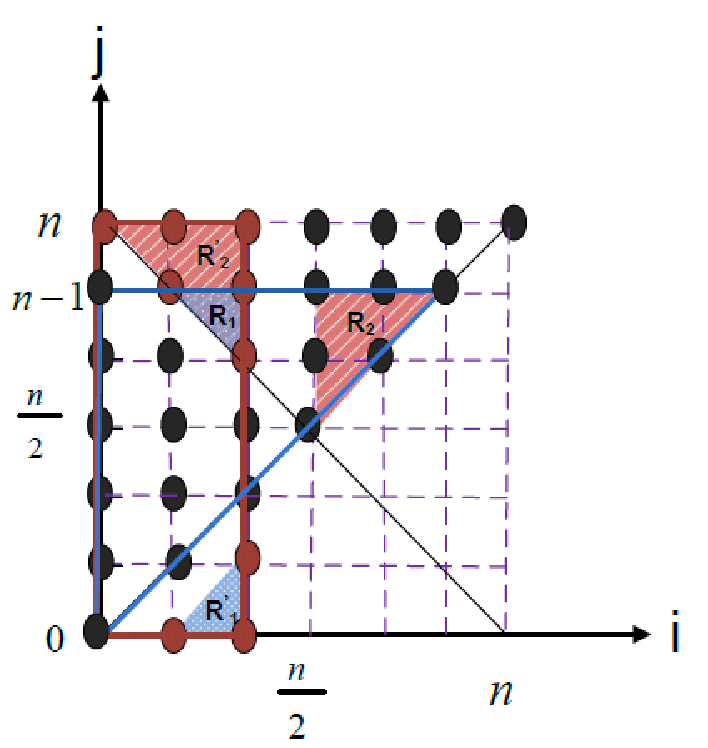
\includegraphics[width=0.45\linewidth]{figtkde/eventransform}
\label{even:subfig1}
}
~~\subfloat[Solution when Grid size n is odd number ]{
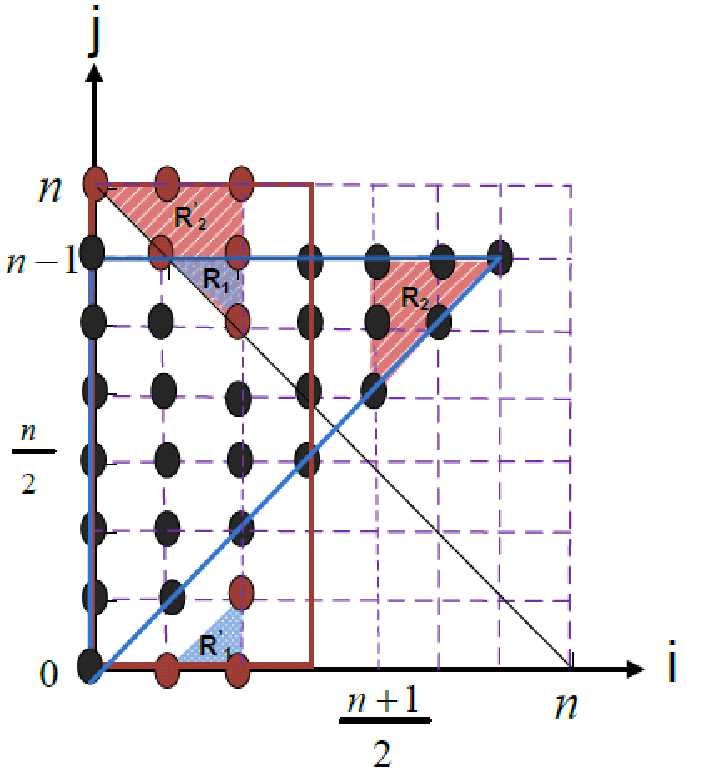
\includegraphics[width=0.45\linewidth]{figtkde/oddtransform}
\label{odd:subfig1}
}
\caption{1-d Interval Transformation from $[n,n]$ to $[\lfloor (n+1)/2 \rfloor,n+1]$}\label{modelBF}
\end{figure}

$\noindent \textit {Example:}$ To illustrate the transformation, Figure~\ref{example:subfig1} and ~\ref{example:subfig2} show small examples on how to transform the intervals when having data points $\{x_0,x_1,x_2,x_3,x_4\}$ and $\{x_0,x_1,x_2,x_3,x_4,x_5\}$ respectively. For data point $(i,j)\in \{x_0,x_1,x_2,x_3,x_4\}$, the total intervals is $10$. By plotting out all of them in Figure~\ref{example:subfig1}, the triangular shaped space is bounded by $(0,0)\rightarrow(3,3)\rightarrow (0,3)$ and there are exactly $10$ points in total. The rectangular shaped space is bounded by $(0,0)\rightarrow(1,0)\rightarrow (1,4)\rightarrow (0,4)$ and total number of points is exactly $10$. Similarly, for data point $(i,j)\in \{x_0,x_1,x_2,x_3,x_4,x_5\}$,  the triangular shaped space is bounded by $(0,0)\rightarrow(3,3)\rightarrow (0,3)$ and total number of points is . The rectangular shaped space is bounded by $(0,0)\rightarrow(1,0)\rightarrow (1,4)\rightarrow (0,4)$ and total number of points is exactly $10$. Table~\ref{maptable} shows the transformations.

\begin{figure}[h]
\centering
\subfloat[ Grid size n =4 ]{
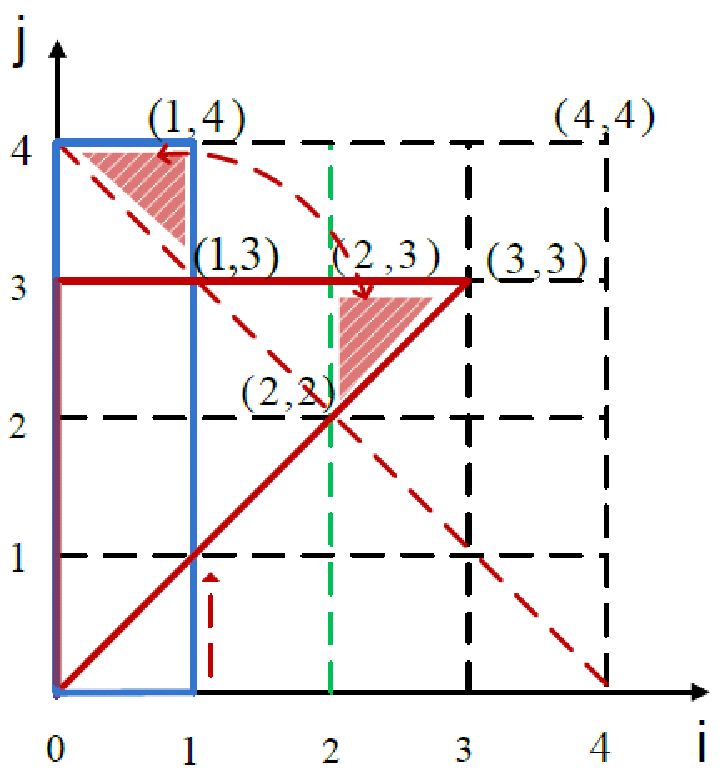
\includegraphics[width=0.45\linewidth]{figtkde/exampleven}
\label{example:subfig1}
}
~~\subfloat[Grid size n =5 ]{
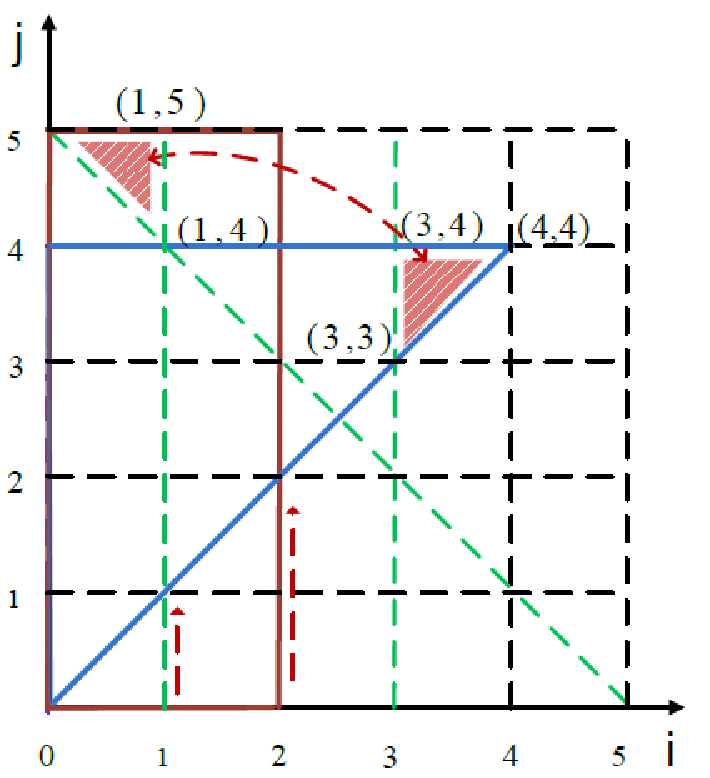
\includegraphics[width=0.45\linewidth]{figtkde/exampleodd}
\label{example:subfig2}
}
\caption{Example: 1-d Interval Transformation}\label{example}
\end{figure}

\begin{table}[!ht]\small
  \centering \small
  \subfloat[Grid (4,4)\label{maptable1}]{
    \centering \small
     \begin{tabular}{|c|c|c|}
	\hline
    (0,0)$\rightarrow (0,0)$  &  $(0,1) \rightarrow (0,1)$&  $(0,2) \rightarrow (0,2)$ \\
    \hline
    (0,3)$\rightarrow (0,3)$  &  $(0,4) \rightarrow (3,3)$&  $(1,4) \rightarrow (2,2)$ \\
    \hline
    (1,3)$\rightarrow (2,3)$  &  $(1,0) \rightarrow (1,1)$&  $(1,1) \rightarrow (1,2)$ \\
    \hline
     (1,2)$\rightarrow (1,3)$  &    &  \\
    \hline

\end{tabular}
  }\\
  \subfloat[Grid (5, 5)\label{maptable2}]{
    \centering \small
   \begin{tabular}{|c|c|c|}
	\hline
    (0,0)$\rightarrow (0,0)$  &  $(0,1) \rightarrow (0,1)$&  $(0,2) \rightarrow (0,2)$ \\
    \hline
    (0,3)$\rightarrow (0,3)$  &  $(0,4) \rightarrow (0,4)$&  $(0,5) \rightarrow (4,4)$ \\
    \hline
    (1,0)$\rightarrow (1,1)$  &  $(1,1) \rightarrow (1,2)$&  $(1,2) \rightarrow (1,3)$ \\
    \hline
    (1,3)$\rightarrow (1,4)$  &  $(1,4) \rightarrow (3,4)$&  $(1,5) \rightarrow (3,3)$ \\
    \hline
    (2,0)$\rightarrow (2,2)$  &  $(2,1) \rightarrow (2,3)$&  $(2,3) \rightarrow (2,4)$ \\
    \hline
\end{tabular}
  }
  \caption{Example: Interval Transformation for even/odd number of points }\label{maptable}
\end{table}

\subsection{Two-Dimensional Mapping}
By extending one-dimensional mapping directly, two-dimensional mapping is given in the following:

\begin{flalign*}
&\mathbb N_k = \{0..n_k-1\}          & \\
&\mathbb R_k = \{0..\frac{n_k}{2}-1\} \times \{0..n_k\}&\\
&\mathbb T_k = \{(a_k,b_k) \in \mathbb N_k^2 | a_i<=b_k\}&\\
&\mathbb M_k = \{0.. \frac{n\times (n_k+1)}{2}-1\}&\\
\end{flalign*}
where $k=1,2$, $N_1,N_2$ are coordinate range , $R_1, R_2$ are rectangular space , $T$ is triangular space  and $M$ is number range.\\


\subsection{k-Dimensional Mapping}
Mapping function $\phi^k: M^k \rightarrow R^k \rightarrow T^k$\\
by using Horner's scheme to transform a number in $M^k$ to a k-dimensional tuple $(x_1, ...,x_k)$. Then we can use mappings $\phi_1$ and $\phi_2$ to do the translation from each element $x_i$ to $(l_i,u_i)$.

\begin{definition}
Mapping Function
\begin{flalign*}
\phi_1^k:  \mathbb M^k \rightarrow \mathbb R^k & \\
x \mapsto (x_1,...,x_k)
\end{flalign*}
 where  $x_k  = x \div (n+1)$ and $b = x \mod (n+1)$.
\end{definition}
 \vspace{5mm}

\begin{algorithm}[t!]\small
\label{RM}
\caption{ Parallel Range Mapping in 1-d array}\label{RM}
Input:  n data points \\
Output: mapping all the intervals from rectangular to triangular space\\
------------------------------------------------------------------ \\
\begin{algorithmic}[1]
\STATE //The interval (i',j') in rectangular space is transformed to interval (i,j) in triangular space
\FOR{\textit i' \(\leftarrow\)0 to \textit{(n+1)/2}}
\FOR{\textit j' \(\leftarrow\)0 to \textit{n}}
\IF{$j'\textless (n-i')$ }
\STATE{\textit i\(\leftarrow\)i'}
\STATE{\textit j\(\leftarrow\)(i'+j')}
\ELSE
\IF{$2(i'+1)\textless (n+1)$ }
\STATE {\textit i\(\leftarrow\)(n-i'+1)}
\STATE {\textit j\(\leftarrow\)(n-j'+i)}

\ENDIF
\ENDIF
\STATE \textit {LRT computation for interval (i,j)}
\ENDFOR
\ENDFOR
\end{algorithmic}
\end{algorithm}

\subsection{Inclusive/Exclusive Pre-computation Scheme}

Motivated by section~\ref{sec:mov2}, to obtain a query time of $\bigo(1)$, we need to pre-compute sets $A$, $B$, $X$, and $Y$ for all possible regions in $G$. Since one of the corner is fixed we can pre-compute the cardinalities of these sets in tables of size $\bigo(n^2)$.

To obtain the tables for $A$, $B$, $X$, and $Y$, we employ dynamic programming. The dependency and statistic counts' propagation of rows and columns for these tables are shown in Figure~\ref{prec:subfig1},~\ref{prec:subfig2},~\ref{prec:subfig3} and ~\ref{prec:subfig4}. For example, the table for $A$ can be computed using the following recurrence relationship:

\small
\begin{equation}
\begin{split}
|A(i,j)|  &= |A(i,j-1)| + |A(i-1,j)| - |A(i-1,j-1)| \\& \quad + |G(i,j)|
\end{split}
\end{equation}
\normalsize
where $|G(i,j)|$ counts whether there is an element in the cell location $(i,j)$. The first element and the first column and row need to be populated (initialized) so that all cardinalities of $A$ can be computed. The counts in the remaining rows and columns are accumulated through the dependency of the previous row and column. Figure~\ref{prec:subfig1} shows the computation of set $A$ and the implementations of it is listed in Algorithm~\ref{pre1} (see the proofs and the rest implementation of set $B,X,Y$ in Appendix.)

Similarly, the computation of set $B,X,Y$ is listed as the following:
\small
\begin{equation}
\begin{split}
|B(i,j)|  &= |B(i+1,j)| + |B(i,j+1)| - |B(i+1,j+1)| \\& \quad + |G(i,j)|
\end{split}
\end{equation}
\normalsize
\small
\begin{equation}
\begin{split}
|X(i,j)|  &= |X(i,j+1)| + |X(i-1,j)| - |X(i-1,j+1)| \\& \quad + |G(i,j)|
\end{split}
\end{equation}
\normalsize
\small
\begin{equation}
\begin{split}
|Y(i,j)|  &= |Y(i+1,j)| + |Y(i,j-1)| - |Y(i+1,j-1)| \\& \quad + |G(i,j)|
\end{split}
\end{equation}
\normalsize

\begin{figure}[h]
\centering
\subfloat[Pre-computation of set A  ]{
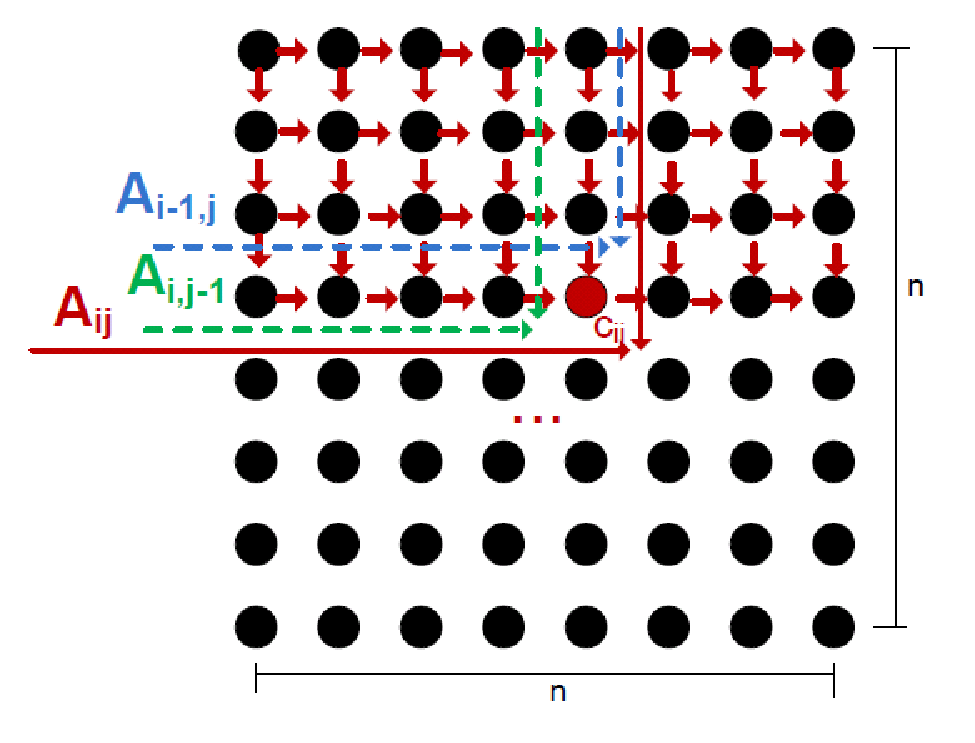
\includegraphics[width=0.4\linewidth]{figtkde/prea}
\label{prec:subfig1}
}
~~\subfloat[Pre-computation of set B]{
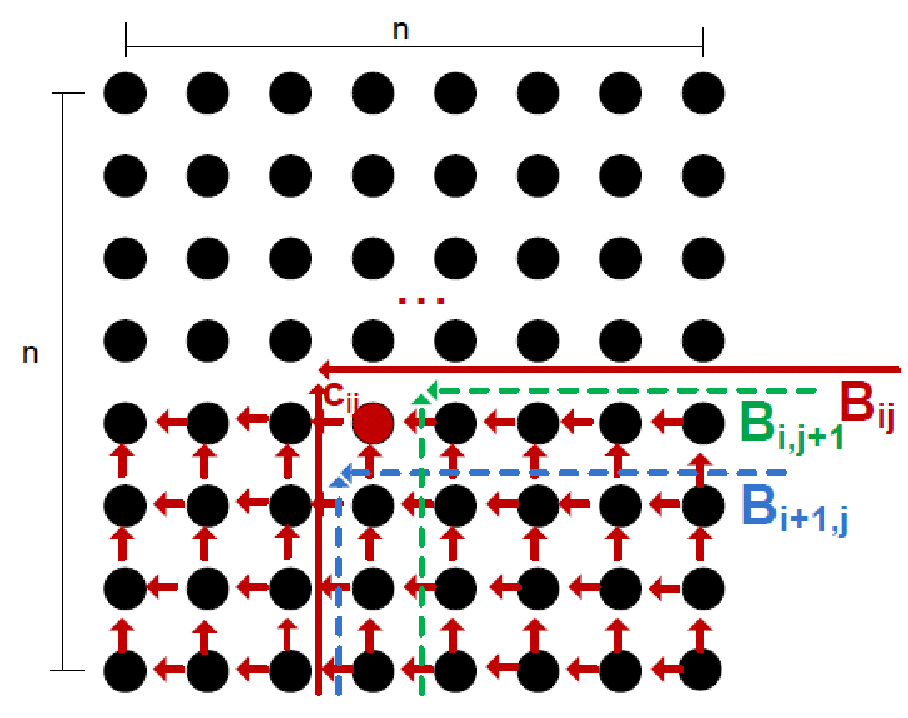
\includegraphics[width=0.4\linewidth]{figtkde/preb}
\label{prec:subfig2}
}\\
~~\subfloat[Pre-computation of set X]{
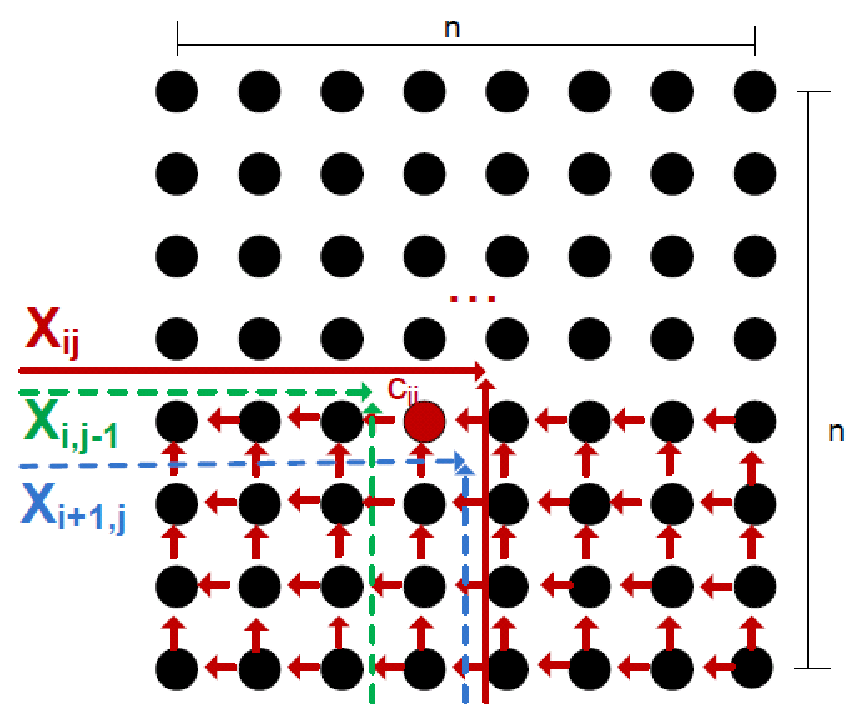
\includegraphics[width=0.4\linewidth]{figtkde/prex}
\label{prec:subfig3}
}
~~\subfloat[Pre-computation of set Y]{
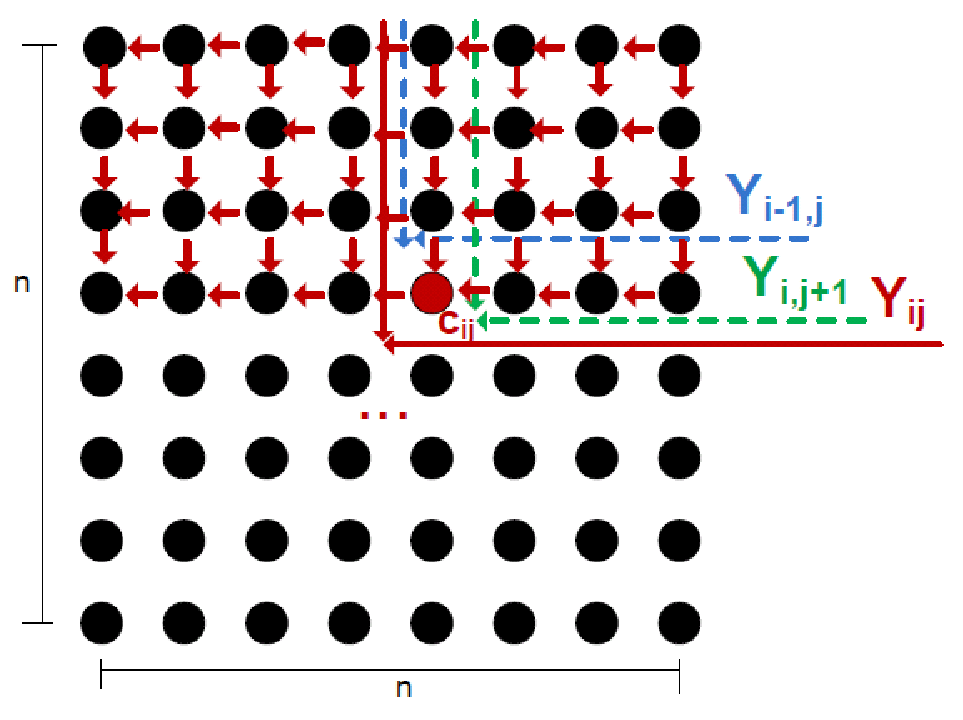
\includegraphics[width=0.4\linewidth]{figtkde/prey}
\label{prec:subfig4}
}
\caption{pre-computation of set A, B, X and Y}\label{prec}
\end{figure}

Due to the high dependency among rows and columns, pre-computing is hard to parallelise and the computation is very fast on a CPU. In our work, the pre-computation of set $A, B, X, Y$ is done on a CPU.


\begin{algorithm}[t!]\small
\label{pre1}
\caption{Inclusive/Exclusive Pre-computation for Set A}\label{pre1}
Input: data grid (G) \\
Output: accumulated counts $A(i,j)$\\
------------------------------------------------------------------ \\
\begin{algorithmic}[1]
\STATE //Initialize first element $A(0,0)$
\STATE {\textit { $A(0,0)$\(\leftarrow\)$G(0,0)$}}
\STATE //accumulation of remaining elements in first row
\FOR{\textit  j\(\leftarrow\)1 to \textit{n}}
\STATE{\textit { $A(0,j)$ \(\leftarrow\) $G(0,j)$ +$A(0,j-1)$}}
\ENDFOR
\STATE //accumulation of remaining elements in first column
\FOR{\textit  i\(\leftarrow\)1 to \textit{n}}
\STATE  {\textit {$A(i,0)$\(\leftarrow\)$G(i,0)$ + $A(i-1,0)$}}
\ENDFOR
\STATE //accumulation of all the elements in remaining rows and columns
\FOR{\textit  k\(\leftarrow\)1 to \textit{n}}
\FOR{\textit  i\(\leftarrow\)k to \textit{n}}
\STATE  {\textit { $A(i,k)$\(\leftarrow\) $G(i,n+k)+A(i-1,k)+A(i,k-1)-A(i-1,k-1)$}}
\ENDFOR
\FOR{\textit  j\(\leftarrow\)k to \textit{n}}
\STATE  {\textit { $A(k,j)$\(\leftarrow\) $G(k,n+j)+A(k,j-1)+ A(k-1,j)-A(k-1,j-1)$}}
\ENDFOR
\ENDFOR
\end{algorithmic}
\end{algorithm}
\end{document}



